\chapter{Stopwatch Datapath and Control}
\label{chapter:swDpAndCu}
\graphicspath{ {./Lab11Stopwatch/Fig} }

\section{Outcomes and Objectives}

The outcome of this lab is complete the implementation
of the stopwatch  on the FPGA development board.
Through this process you will achieve the following
learning objectives.
\begin{itemize}
	\item \Paste{bok:DaC_Architecture}
	\item \Paste{bok:DaC_Timing}
	\item \Paste{HDL:Synthesis}
\end{itemize}



\section{Stopwatch}

From the previous lab, you should be familiar with the operation of our
stopwatch. Briefly, our stopwatch allows a user to measure elapsed time
and lap times of a competitive events. Our stopwatch measures time in
increments of a tenth of a second, unit second and tens of seconds.
Control input comes from 2 buttons called S1 and S2 according to the
finite state machine shown in Figure~\ref{fig:swHighLevel}.

\begin{figure}[ht]
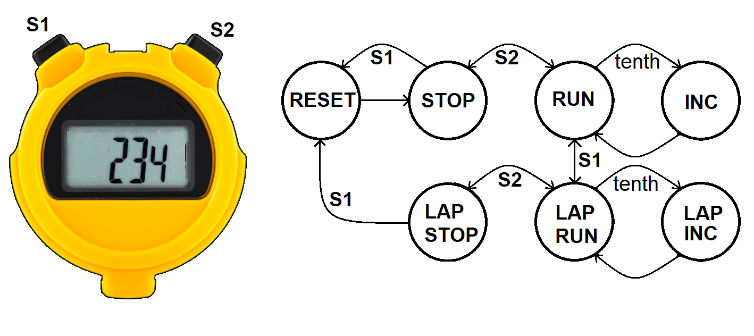
\includegraphics{image1.png}
\caption{A digital stopwatch gets its input from 2 buttons and displays
its output on a 7-segment display. The behavior of the stopwatch can be
described by this finite state machine (FSM).}
\label{fig:swHighLevel}
\end{figure}

Figure~\ref{fig:swDevBoard} shows how you will implement the idea presented in Figure~\ref{fig:swHighLevel}
using the FGPA development board.

\begin{figure}[ht]
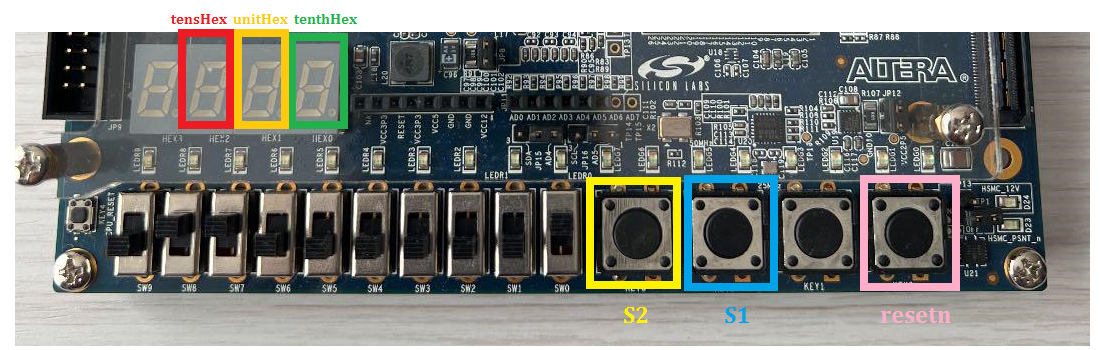
\includegraphics{image2.png}
\caption{The stopwatch user interface as implemented on the FPGA
development board.}
\label{fig:swDevBoard}
\end{figure}

Two of the buttons will act as the stopwatch buttons
and 3 of the 7-segment displays will show the time. The reset signal is
connected to a button and the 50MHz clock is on the FPGA
development board but does not require any user
interaction.

\section{System Architecture}

In the previous 2 labs you have created the datapath and control unit
for the stopwatch. Using these 2 components as building blocks, the
architecture for the stopwatch, shown in Figure~\ref{fig:swArch}, is almost trivial;
the Verilog file for the stopwatch contains 2 component instantiations
of the datapath and controlUnit.

\begin{figure}
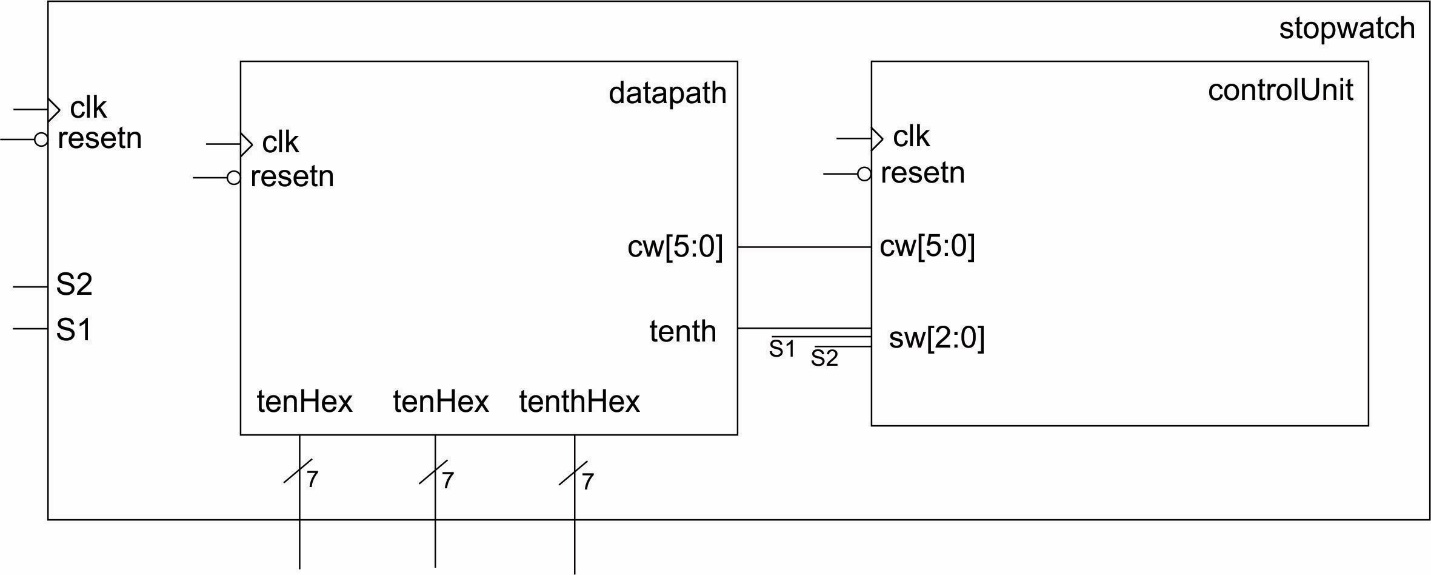
\includegraphics{image3.jpeg}
\caption{The architecture for the stopwatch consists of a datapath and
controlUnit.}
\label{fig:swArch}
\end{figure}

The only minor complication is combining the tenth output from the
datapath with the S2 and S1 signals coming in from the
buttons into a 3-bit signal sent to the status word input of the control
unit.

Use the starter code provided on Canvas to complete the stopwatch
module. While you are at it, download the stopwatch testbench provided
on Canvas, and make the testbench the top-level entity.

\subsection{Testbench}

Before you download your completed control unit to the development boards,
you are going to perform extensive simulations to uncover as many bugs
as possible. Errors are much, much easier to find in a simulation. First
you will need to understand what the testbench simulation is supposed to
do.

The timing diagrams in Figure~\ref{fig:swTiming} show the S1 and S2 signals
as they are manipulated by the testbench. The tenth signals will be
asserted by your datapath but are included to help you. Your task is to
fill in the symbolic name of the state that the FSM is in as well as the
clkCount value, the mod10Counter outputs and the values displayed on the
7-segment displays.

\begin{landscape}

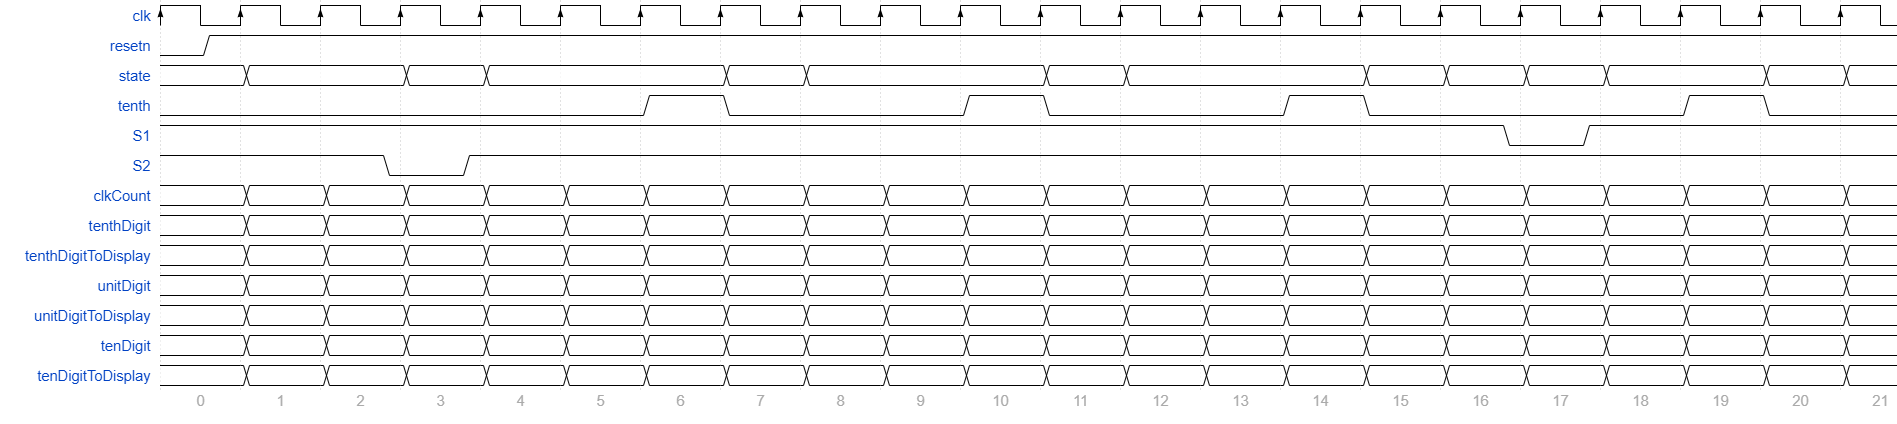
\includegraphics{image5.png}

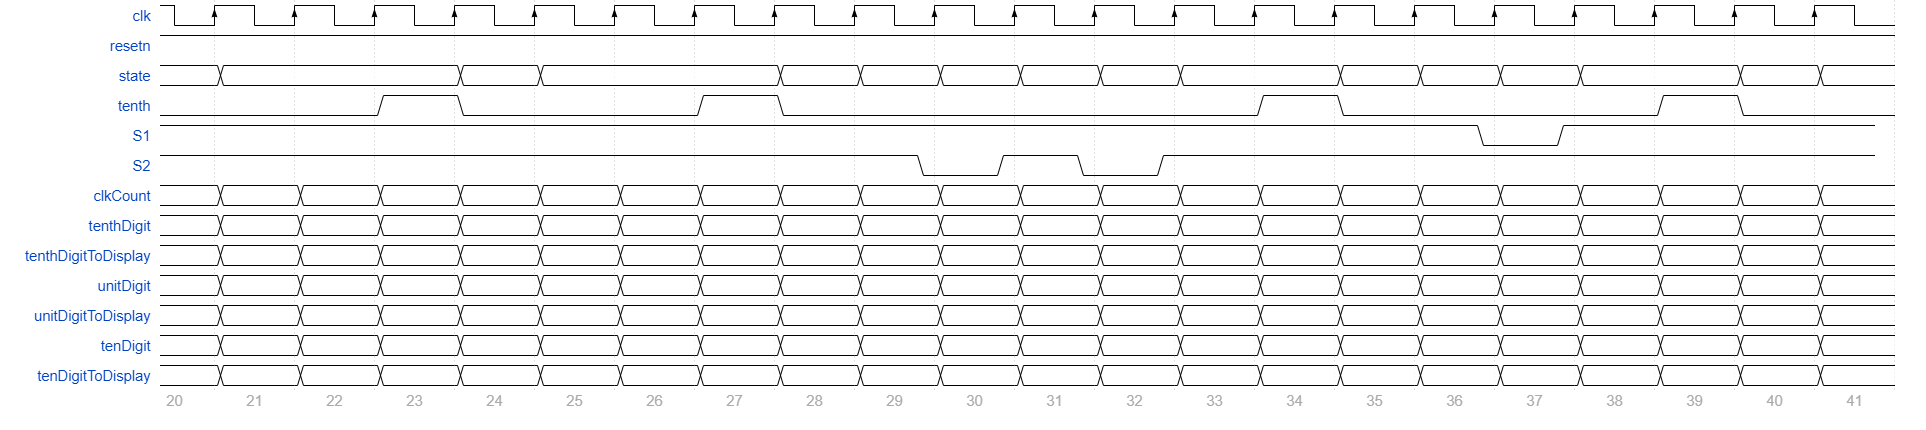
\includegraphics{image6.png}
\begin{figure}
\caption{Timing diagram that you will run on the testbench.}
\label{fig:swTiming}
\end{figure}
\end{landscape}

The goal of the testbench was to cover every transition arc in the state
diagram. This goal was not achieved; several transition arc was not
taken in the testbench, which one was it? I'd suggest double checking
this transition during the testing of the stopwatch when it is
downloaded onto the FPGA development board.

\hypertarget{link:swTestbench}
Run the testbench using the provided do file and compare the output
against Figure~\ref{fig:swTiming} You will probably need to modify the do
file to make it work with your design. Address any problems in the
stopwatch before proceeding.

\subsection{Pin-Assignment and Synthesis}

When you created the datapath, you intentionally designed the timer
counter to count up from 0 to 2 in order to expedite execution of the
simulations. Before you synthesize the datapath, you need to undo this.
I would suggest leaving the relevant constants in your code and just
comment them out. Immediately following each commented constant, put the
constant that you need for the datapath to operate correctly on the
FPGA development board. I've summarized these changes in Listing~\ref{listing:swtenthSecond}.

\begin{lstlisting}[language=Verilog,
 caption={Changes to the datapath that will allow it to run properly on the FPGA development board.},
 label={listing:swtenthSecond},
 frame=single]
// parameter N = 4;	
parameter N = 24;	

// localparam   tenthSecondConstant   = 4'h000002;
localparam   tenthSecondConstant   = 24'h4c4b40;

//localparam   zero24 = 4'h000000;
localparam   zero24 = 24'h000000;
\end{lstlisting}


While you are at it, make sure that you remove the testbench as the
top-level module and make the stopwatch the top-level module. Then run
the analysis and elaboration tool to make sure that the changes in
Listing~\ref{listing:swtenthSecond} did not create any warnings or errors

The next step is to create the mapping of stopwatch module inputs and
outputs to the pins of the FPGA and by extension the input and output
devices on the FPGA development board. Use the inputs and outputs shown in
Figure~\ref{fig:swDevBoard} and the information in the FPGA development board User Guide to complete
the following pin assignment tables.

\begin{longtable}[]{@{}
| >{\raggedright\arraybackslash}p{(\columnwidth - 4\tabcolsep) * \real{0.3334}}|
  >{\raggedright\arraybackslash}p{(\columnwidth - 4\tabcolsep) * \real{0.3334}}|
  >{\raggedright\arraybackslash}p{(\columnwidth - 4\tabcolsep) * \real{0.3333}}|@{}}
  \caption{Pin assignment for the stopwatch.}\label{table:swPinAssignment}\tabularnewline
\toprule()
S2 & Key{[}3{]} & Y16 \\
\midrule()
\endhead
S1 		& Key{[}2{]} 		& \\ \hline
resetn	& Key{[}0{]} 		& \\ \hline
clk		& CLOCK\_50 	& R20 \\
\bottomrule()
\end{longtable}

\begin{longtable}[]{@{}
| >{\raggedright\arraybackslash}p{(\columnwidth - 6\tabcolsep) * \real{0.1548}}|
  >{\raggedright\arraybackslash}p{(\columnwidth - 6\tabcolsep) * \real{0.2313}}|
  >{\raggedright\arraybackslash}p{(\columnwidth - 6\tabcolsep) * \real{0.2323}}|
  >{\raggedright\arraybackslash}p{(\columnwidth - 6\tabcolsep) * \real{0.3816}}|@{}}
\toprule()
\begin{minipage}[b]{\linewidth}\raggedright
Segment
\end{minipage} & \begin{minipage}[b]{\linewidth}\raggedright
tenHex Hex2
\end{minipage} & \begin{minipage}[b]{\linewidth}\raggedright
unitHex Hex1
\end{minipage} & \begin{minipage}[b]{\linewidth}\raggedright
tenthHex Hex0
\end{minipage} \\
\midrule()
\endhead
seg{[}6{]} & & & \\ \hline
seg{[}5{]} & & & \\ \hline
seg{[}4{]} & V20 & & \\ \hline
seg{[}3{]} & & & \\ \hline
seg{[}2{]} & & & V17 \\ \hline
seg{[}1{]} & & & \\ \hline
seg{[}0{]} & & AA18 & \\
\bottomrule()
\end{longtable}

After making the pin assignment, download and test your design.

\section{Turn in}

You may work in teams of at most two. Make a record of your response to
the items below and turn them in a single copy as your team's solution
on Canvas using the instructions posted there. Include the names of both
team members at the top of your solutions. Use complete English
sentences to introduce what each of the following listed items (below)
is and how it was derived. In addition to this submission, you will be
expected to demonstrate your circuit at the beginning of your lab
section next week.

\subsubsection{Testbench}

\begin{itemize}
\item
  Completed Figure~\ref{fig:swTiming}. Please paste the images in landscape format into your solutions

\item
  Screen shot of \hyperlink{link:swTestbench}{simulation timing diagram}. Please compose the simulation in landscape 
  format into your solutions and break the screen shot of the simulation into three parts,

  \begin{itemize}
    \item
      from 0 to 400ps
    \item
      from 400ps to 800ps
    \item
      from 800ps to 1200ps
\end{itemize}
\end{itemize}

\subsubsection{Pin-Assignment and Synthesis}

\begin{itemize}
\item
  Completed pin assignment from Table~\ref{table:swPinAssignment}.
\item
  Demonstrate your working stopwatch to a member of the lab team.
\end{itemize}
